\documentclass[12pt]{paper}
%\usepackage{paper} %if the document does not compile properly for you on the initial build, uncomment \usepackage{paper} and build again. This should force MikTeX to install package "paper"
\usepackage[margin=1in]{geometry}
\usepackage{float}
\usepackage{natbib}
\bibliographystyle{apsr}
\usepackage{graphicx}
\graphicspath{ {../fig/} }
\usepackage{setspace}
\usepackage[super]{nth}
\usepackage{booktabs}
\usepackage{makecell}
\usepackage{amsmath}
\usepackage{dcolumn}
%\usepackage{authblk}
\usepackage{hyperref}
\usepackage{wrapfig}
\usepackage{amsmath}
\usepackage{adjustbox}
%\usepackage{etoolbox}
%
%\AtBeginEnvironment{quote}{\singlespacing\small}
%\usepackage{epigraph}

\begin{document}

\title{Give a Man a Fish and He'll Eat for a Day, But Will He Vote for You?: A Formal Approach to Federal Redistribution and Voter Behavior}
\author{Sarah R. Warren}
\date{\today}
\maketitle
%\epigraph{QUOTE}{\textit{ATTRIBUTION}}
\setstretch{2}
%\thispagestyle{empty}
%\clearpage
%\setstretch{1}


%%QUOTE ABOUT VOTES AND DEMOCRACY

\section{Introduction}
The popular vote is one of the most important aspect of democracy. It is the means by which voters attain representation (SOURCE) and then hold representatives accountable (SOURCE). But who is represented and who holds representatives accountable depends on who votes. It is well-established that voters with higher education and income turnout more often than their lower-resourced counterparts (Wolfinger and Rosenstone 1980). Public assistance recipients are an especially quiescent voting bloc (Verba, Schlozman, and Brady 1995). 47\% of eligible adults with family incomes of less than \$20,000 a year voted in 2012 and just 25\% voted in the 2010 midterm elections. Consequently, voter participation is among the most widely studied components of political behavior. Scholars have long considered the individual, social, and systemic factors that influence the decision to show up to the polls on election day. 

Seymour Lipset (1960) argued that one's decision to vote depends upon the perceived “relevance of government policies to the individual.” Modern theories of voting behavior still rely on Lipset’s (1960) summation of the boundedly rational political actor: voters turnout based on the perceived relevance of politics to their own lives (Conover, Feldman, and Knight 1986; Conover, Feldman, and Knight 1987; Dowding 2005; Fedderson and Sandroni 2006; Hansford and Gomez 2015). Thus, what matters is not simply the objective relevance of government to the voter, but the extent to which government agents can effectively claim credit (or avoid blame) for governmental action that citizens perceive to affect them. Presumably, then, those who stand to benefit the most from generous government policies (and, conversely, be most harmed by social spending cuts) should be likely to vote. Unlike government redistribution in the form of roads, fire and police protection, social welfare benefits are often targeted, direct money-transfers from a federal or state office to an individual or household in need. Public aid beneficiaries have an unusually visible stake in election and policy outcomes, particularly if they participate in aid programs that assist in feeding their families, providing health insurance, and meeting other immediate, tangible needs. In this case, public funding priorities have a direct impact on the quality and quantity of food, healthcare, and spending money these households receive.

Given such strong personal incentives, one might expect welfare recipients to be more politically active than other citizens (Lipset 1960; Olson 1965); however, this does not appear to be the case in the United States. As political scientists, how can we reconcile our theoretical predictions with this empirical reality? I build on existing theories of attribution and voter behavior to model a novel theoretical explanation for the voting behavior of American welfare recipients. I empirically evaluate the implications of my model using data from the Maxwell Poll from 2004-2007. Using a novel measurement technique to classify aid-types, I find that entitlements are associated with an increase in self-reported turnout in elections while government subsidized loans are associated with a decrease in self-reported turnout. Importantly, the effect of means-tested aid on government turnout appears to be less straightforward than previous work suggests.

I use a dynamic Bayesian model with incomplete information to highlight partisanship as a mechanism which can cause variation in turnout among aid recipients. Having done so, I develop hypotheses which will hold if this model is useful as a picture of the world (CITE JIM AND RUBENSTEIN). I then briefly present an expanded version of the model and test the effects of aid on self-reported self-efficacy. The rest of the paper proceeds as follows. Section 1 reviews the relevant literature and dominant theories of voter attribution and redistributive politics in the United States. Section 2 outlines the model and present its equilibrium outcome. Section 3 presents my empirical hypotheses, data, and empirical analysis. Section 4 presents a brief discussion of the expanded model and an empirical test of the self efficacy mechanism. Section 5 concludes and discusses directions for future research.

\section{The Quiescence of Aid Recipients}
There are two widely accepted reasons for the quiescence of aid-receiving voters in the United States. First, because aid recipients are often less well educated and less well off financially, the boost to their participation by their larger interest in government activity is insufficient to overcome their other resource deficits (Verba, Scholzman, and Brady 1995, 411). Second, aid institutions in the United States diminish the perceived self-efficacy of aid-recipients, making them less likely to turnout to vote. Pateman (1970) and Piven and Cloward (1971) highlight the educative effects of institutions, which shape the behavior of aid participants. Soss (1999) and others (Madsen 1986; Mettler and Stonecash 2008) argue that institutions like means-testing and constant eligibility evaluation by bureaucrats may teach participants that government is not responsive to them. Participants carry a sense of low self-efficacy to other political processes, including as voting, leading to decreased turnout. Other scholars, however, find that aid intended for the very poor can have a very positive effect on political participation (SOURCES).

Some models (Fiorina 1981, 5; Kinder and Kiewiet 1981) suggest that voters choose presidential candidates based on their own financial circumstances, via “pocketbook voting.” In these attributive models, voters take stock of factors such as their personal employment, their health benefits, their income, and other changes to their personal financial situation. Based on these, voters either blame the incumbent for their bad circumstances or credit him with their good circumstances. Other models (Goren 1997; Gomez and Wilson 2001) suggest that voters are sociotropic, or base their economic attributions on national economic factors, such as the GDP, the stock market, inflation, and the unemployment rate. In these models, voters retrospectively blame the incumbent president for rising unemployment and inflation, a falling GDP, and rising taxes.  However, economic voters may be heterogeneous in their response to information. Weatherford (1978) finds that pocketbook responses vary by social class. Conover, Feldman, and Knight  (1986) find that voters differ in the quantity and quality of information they have on the national economy and how they apply it. CFK find that the accuracy of retrospective assessments depends jointly on the availability of information about the issue, the salience of the issue, and the sensitivity of the issue to specific knowledge. Similarly, Hansford and Gomez (2015) find that economic evaluations are colored by appraisals of the incumbent and thus do not operate as an exogenous influence on votes. Thus, the decision to vote and for whom to vote as the joint product of the information about the costs and benefits of voting and how that information is processed. Differences in “processing” most often manifest through partisanship, education, or political sophistication (Gomez and Wilson 2001; Arceneaux 2006; Chen 2013). 

These conventional models of voter behavior and motivation speak to the processes which undergird all voter decisions, but social welfare (1) can impose a unique set of costs on participants through means-testing, (2) can confer a uniquely salient set of benefits through cash transfers or subsidization, (3) and can mitigate the type and salience of economic information recipients process. My novel theory of aid-related voting behavior addresses these contradictory literatures by incorporating the heterogeneous effects for partisanship into the model, as well as allowing the cost of voting to vary across voters.

\section{A Formal Model of Aid and Attribution}
\emph{Players:} Two politicians, an incumbent (I) and a challenger (C), who have different ideal points $(x_I=1, x_C=0)$. A voter (V) whose ideal point $x_V \epsilon [0,1]$ lies somewhere between $x_I$ and $x_C.$

\emph{Player Types:} Nature selects the politicians’ types, $\theta_I,\theta_C \epsilon {0,1}$, with probabilities: $Pr(\theta_I=0)=Pr(\theta_I=1)=Pr(\theta_C=0)=Pr(\theta_C=1)= \frac{1}{2}$ Nature privately reveals $\theta_I,\theta_C$ to I and C, respectively. Type $\theta=0$ prefers not to deliver aid the voter though delivers aid with some positive probability. Type $\theta=1$ prefers to deliver aid though fails to deliver aid with some positive probability. The probability that the politician delivers aid in accordance with his type is $p > 1 – p$ or $p > \frac{1}{2}$

\emph{Sequence of Play}
\begin{enumerate}
	\item Nature determines each politician’s type, $\theta_I, \theta_C \epsilon {0,1},$ with probabilities $(\frac{1}{2}, \frac{1}{2})$ and reveals types privately to I and C, respectively.
	\item Nature draws from the incumbent’s urn to pick the first period aid amount, $y_1\epsilon {0,1}.$ The incumbent responds according to his type with greater likelihood than not. First period aid $y_1\epsilon {0,1}$ is administered.
	\item Nature determines the cost of voting, $c~U[0,1]$ and reveals this cost to voter V.
	\item The voter V chooses whether to vote, $v\epsilon{0,1}$
	\item If V votes $(v=1)$, then he decides the election winner, I or C. If V does not vote $(v=0)$, Nature decides the election winner, I or C.
	\item The winner (I or C) picks the second period aid amount, $y_2\epsilon {0,1}$. The winner responds according to his type with greater likelihood than not. Second period aid  $y_2 \epsilon {0,1}$ is administered.
\end{enumerate}

\emph{Politicians' Utility}: In each period $t\epsilon{1,2}$, each politician $p\epsilon{I,C}$ receives: 

$U_{p}^t = -|\theta_p - y_t|$

where $y_t\epsilon {0,1}$ is the executive’s choice of distributive aid policy. $\theta_p$ denotes the politician’s type, which represents her preferred distributive policy. Hence, a politician of type $\theta_p=1$ prefers to deliver aid $(y_t=1)$, while a politician of type $\theta_p=0$ always prefers no aid $(y_t=0).$

\emph{Voter's Utility}: V’s utility function is constant across periods: 

$U_{V}^t = -|x_o - x_V| + y_t$

where $y_t\epsilon{0,1}$ represents the amount of distributive aid awarded to the voter in period $t\epsilon{1,2},$, $x_V$ represents the voter’s ideal point, and $x_o$ is the ideal point of the office-holding politician, who is either the Incumbent $(x_I=1)$ or the Challenger $(x_C=0).$ Hence, the voter’s utility depends on his ideological proximity to the office holder as well as his benefit from any distributive aid.

In between the two periods, the voter may choose to vote in the election by incurring a turnout cost, $c$, which is randomly drawn by Nature from the uniform distribution $c~U[0,1]$ and revealed to $V$ prior to the election. $V$’s payoff for the entire game is therefore given by:

$U_{V}^1 + U_{V}^2 - c \times v$

where $v\epsilon{0,1}$ is V’s choice of whether to turn out in the election, and $U_{V}^1$ and $U_{V}^2$ are V’s payoffs from the first and second periods, respectively.

\emph{Voter Beliefs}: The Voter V does not observe the politician types, $\theta_I$ and $\theta_C$, that Nature randomly chooses. Instead, V can only observe the Incumbent's first-period distributive policy,  $y_1$, and form updated beliefs about I’s type. Let $p_(\theta_I ) (\theta_p | y_1 )$ denote the V’s posterior beliefs about the probability that $\theta_I=1$ after observing $y_1$.

\subsection{Equilibrium Outcomes}
	For simplicity, I assume that Voter V resolves indifference in favor of abstaining.
	
\textbf{Lemma A (Executive’s Distributive Policy):} In each period $t\epsilon{1,2}$, the office-holding executive, $p\epsilon{I,C}$, chooses the distributive policy: 

$x_t=\theta_j (1-p)+ \theta_i (p)$, 

where $\theta_j$ is the opposite of the office holder’s type. Incumbent types are therefore not fully separating. 


\textbf{Lemma B (Voter’s updated beliefs about Incumbent’s type):}  After observing the Incumbent’s choice of $y_1 \epsilon {0,1}$ during the first period, the Voter V’s updated belief about the Incumbent’s type is: $p_(\theta I) (p(\theta_i ) + (1 - p)(\theta_j ) | y_1 )=y_1$.

Given Lemma B, V expects to receive $E(y_2 | e=I)=p(\theta_i )+(1-p)(\theta_j)$ units of aid in $t=2$ if I is reelected and $E(y_2 |e=C)=E(\theta_C )=\frac{1}{2}$ units of aid if C wins the election.  V’s expected second period payoff from I’s reelection would be: $EU_V (e=I) = -(1 - x_v ) + [p(y_1 ) + (1 - p)(y_1 )]$ whereas his expected second period payoff from C’s election would be: $EU_V (e=C) = - x_V + \frac{1}{2}$. Therefore, conditional on turning out, V votes for I iff: 

$EU_V (e=I) \geq EU_V (e=C) \Rightarrow = -(1 - x_V ) + [p(y_1 ) + (1 - p)(y_1 )] \geq - x_V + \frac{1}{2} \Rightarrow x_V \geq \frac{3}{4} + \frac{p(y_1 - y_-1 ) + y_-1}{2}$

When $x_V$ is above this threshold, V prefers that the Incumbent win the election, so V’s total expected payoff from voting would be:
$ EU_V (v=1 | x_V \geq \frac{3}{4} + \frac{p(y_1 - y_-1 ) + y_-1}{2}) = - (1 - x_V ) + y_1 - c$

When $x_V$ is below the threshold, V prefers that the Challenger win the election, so V’s total expected payoff from voting would be:
$ EU_V (v=1 | x_V \geq \frac{3}{4} + \frac{p(y_1 - y_-1 ) + y_-1}{2}) = -x_V + \frac{1}{2} - c$

In both cases, V’s total combined expected payoff from not voting is:
$ EU_V (v=0) = \frac{EU_V (e=I)}{2} + \frac{EU_V (e=C)}{2} + \frac{- (1 - x_V ) + y_1}{2} + \frac{-x_V + \frac{1}{2}}{2} = \frac{y_1}{2} - \frac{1}{4}$

Hence, in equilibrium, V turns out to vote iff: $EU_V (v=1) \geq EU_V (v=0) \Rightarrow c \leq \bar{c}$ where:

\begin{equation}
\bar{c} =
\begin{cases}
\frac{-y_1}{2} - x_V + \frac{3}{4} & if x_V < \frac{1}{4}\\    
x_V (2y_1 - 1) + \frac{3}{4}     & if \frac{1}{4} \leq x_V < \frac{3}{4}  \\
\frac{y_1}{2} + x_V - \frac{3}{4}     & if x_V \geq \frac{3}{4}  \\
\end{cases}
\end{equation}

\textbf{Lemma C: (V’s Turnout and Vote Choice):} Let $Q_(y_1 )(x_V )$ denote the probability of turnout for a voter with ideal point $x_V$ and who receives $y_1 \epsilon {0,1}$ of aid during Period 1. V’s turnout choice in the election is:

\begin{equation}
Q_(y_1 )(x_V ) =
\begin{cases}
\frac{-y_1}{2} - x_V + \frac{3}{4} & if x_V < \frac{1}{4}\\    
x_V (2y_1 - 1) + \frac{3}{4}     & if \frac{1}{4} \leq x_V < \frac{3}{4}  \\
\frac{y_1}{2} + x_V - \frac{3}{4}     & if x_V \geq \frac{3}{4}  \\
\end{cases}
\end{equation}

Therefore, given turning out, V’s vote in the election is:
\begin{equation}
s =
\begin{cases}
I, & if x_V \geq \frac{3}{4} + \frac{p(y_1 - y_-1) + y_-1}{2} \\    
C,     & otherwise  \\
\end{cases}
\end{equation}
where $y_-1$ is the aid amount not delivered in the period (i.e. if $1$ unit of aid was delivered, $y_-1 = 0$.)

Given this, we can calculate the \emph{change in turnout probability} from receiving one unit of aid in $t_1$. Put differently, the effect of receiving $y_1 = 1$ is:
\begin{equation}
Q_1 (x_V ) - Q_0 (x_V )=
\begin{cases}
\frac{-1}{2} & if x_V < \frac{1}{4}\\    
2x_V - 1 & if \frac{1}{4} \leq x_V < \frac{3}{4}  \\
\frac{1}{2} & if x_V \geq \frac{3}{4}  \\
\end{cases}
\end{equation}

In other words, delivering aid to ideologically distant voters $(x_V < \frac{1}{2})$ strictly decreases their probability of turning out, while delivering aid to ideologically proximate voters $(x_V > \frac{1}{2})$  strictly increases their probability of turning out. Additionally, conditional upon turnout, delivering aid strictly increases the likelihood of voting for the incumbent. The delivery of aid during period one increases V’s expected payoff from having the incumbent reelected relative to the probability that the aid distribution was an informative signal. The increased expected payoff drives my main prediction that the delivery of aid in period one increases a right-wing voter's probability of turnout.

\begin{figure}
	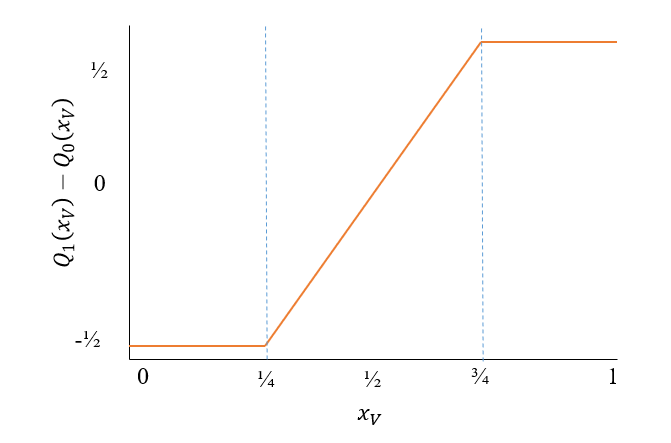
\includegraphics[width=\linewidth]{Figs/equilibrium.png}
	\caption{Figure 1: Change in Turnout Probability Given Aid}
	\label{Figure 1: Change in Turnout Probability Given Aid}
\end{figure}

From Lemmas A, B, and C, we can derive the simple prediction that those who favor the incumbent \emph{a priori} credit the Incumbent with the positive experience of aid and, therefore, turnout to vote for him or her. Those who do not favor the incumbent \emph{a priori}, rather than change their vote choice, are simply less motivated to turnout to oust the Incumbent. Distant voters, therefore, should be less likely to turnout to vote at all. Put differently, receiving aid in $t_1$ causes a relatively larger increase in a right-wing voter’s turnout probability but a relatively smaller decrease in a left-wing voter’s turnout probability, given $p > \frac{1}{2}$. 

\emph{H1(a): For a left-wing voter $(x_V < \frac{1}{2})$, receiving distributive aid in period 1 causes a strict decrease in the probability of voter turnout.}

\emph{H1(b): For a right-wing voter $(x_V > \frac{1}{2})$, receiving distributive aid in period 1 causes a strict increase in the probability of voter turnout.}

\section{Research Design}
To test the implications of my model, I utilize data from The Maxwell Poll on Citizenship and Inequality from Syracuse University, directed by Jeffery Stonecash. The poll includes data on federal aid status, voter behavior, and civic engagement. The poll is nation-wide annual survey and was administered by phone from 2004-2007. The cumulative data file from the surveys contain weights so that the data is nationally representative and each year averages approximately 600 respondents (n=458-480 after controlling for null responses in the data).

I conduct my analysis using binary and ordered logit models, but my results are robust to OLS estimation (see Appendix). My dependent variable is turnout. The Maxwell Poll asks respondents whether they turnout Always (4), Often (3), Sometimes (2), or Not at all (1). I use this ordinal measure of turnout as well as a binary measure in which those who respond ``Always" and ``Often" are coded 1 and those who responded ``Sometimes" and ``Never" are coded 0.

My primary independent variable is receiving government aid. I employ several measures of aid in different models to account for heterogeneity within aid programs and account for the cumulative effect of aid on voter behavior. First, I use binary variables for each of the nineteen aid programs contained in the Maxwell Poll dataset in which a 1 means the respondent or a member of the respondent’s household receives the benefit and a 0 means no one in the household receives that benefit. Second, I create a binary variable in which 1 means the respondent or a member of the respondent’s household receives any form of government assistance and a 0 means no one in the household receives government aid. Finally, I use counts of the total number of entitlement, means-tested, universal, and subsidized loan aid the household receives to create an aid-category participation measure. A 0 in all four categories would mean the respondent’s household receives no aid, while a 1 in entitlements and a 0 in the other three categories would mean the respondent’s household receives one kind of entitlement benefit, but no other government aid.

My theory predicts that Party ID directly influences voting behavior after aid. I use a binary measure in which a 1 is Republican and a 0 is Democrat. I also include a battery of controls, including race, income, education, sex, how closely the person follows public events, their trust in public officials, and their sense of their political self-efficacy.

\section{Analysis}
First, I estimate a model using dummy variables for each aid program. Recall that my model shows that, holding partisan affiliation constant, aid has a strictly positive effect on the probability of turnout. This model estimates the effect of each aid program on voting frequency, holding all else constant.

In the binary logit, Social Security, Unemployment Insurance, and Mortgage Tax Credits have a positive and significant effect on the likelihood of turnout, holding all else constant. Medicaid, Medicare, and Head Start has a negative effect, holding all else constant. In the ordered logit, EITC and Head Start have a negative and significant effect on turnout and Social Security Disability Insurance has a positive and significant effect on turnout, holding all else constant. In both models, controls behave largely as expected, except for Following Public Affairs. Following public affairs is associated with a \textit{decrease} in the likelihood of turning out.

%%Model 2: Vote ~ all programs + controls (race, income, education, sex, followpa, trustoff, peopsay)
\newgeometry{left=3cm,bottom=0.5cm,right=3cm,top=0.5cm}
	\begin{table}[!htbp] \centering 
		\small
		\begin{adjustbox}{width=.6\textwidth}
			\begin{tabular}{@{\extracolsep{5pt}}lD{.}{.}{-3} D{.}{.}{-3} } 
				\\[-1.8ex]\hline \\[-1.8ex] 
				\\[-1.8ex] & \multicolumn{1}{c}{Vote Frequency Dummy} & \multicolumn{1}{c}{Vote Frequency (1-4)} \\ 
				\\[-1.8ex] & \multicolumn{1}{c}{Binary Logit} & \multicolumn{1}{c}{Ordered Logit} \\ 
				\\[-1.8ex] & \multicolumn{1}{c}{(1)} & \multicolumn{1}{c}{(2)}\\ 
				\hline \\[-1.8ex] 
	PTYIDd & 0.499 & 0.036 \\ 
	& (0.492) & (0.228) \\ 
	white & 0.092 & 0.100 \\ 
	& (0.550) & (0.269) \\ 
	EDUC & -0.104 & 0.011 \\ 
	& (0.233) & (0.113) \\ 
	sex & -0.143 & -0.018 \\ 
	& (0.454) & (0.232) \\ 
	FOLLOWPA & -0.992^{***} & -0.814^{***} \\ 
	& (0.240) & (0.127) \\ 
	TRUSTOFF & 1.570^{***} & 0.397^{*} \\ 
	& (0.469) & (0.225) \\ 
	PEOPSAY & 1.333^{***} & 0.106 \\ 
	& (0.482) & (0.236) \\ 
	FDSTMPd & -1.084 & 0.176 \\ 
	& (0.945) & (0.572) \\ 
	SOCSECd & 4.143^{***} & 0.499 \\ 
	& (1.522) & (0.497) \\ 
	MEDAIDd & -1.519^{*} & -0.623 \\ 
	& (0.889) & (0.471) \\ 
	MEDICAREd & -2.591^{**} & -0.387 \\ 
	& (1.231) & (0.539) \\ 
	WELFAREd & -0.599 & -0.038 \\ 
	& (0.971) & (0.531) \\ 
	EITCd & -0.292 & -0.496^{**} \\ 
	& (0.514) & (0.245) \\ 
	UNEMPLOYd & 1.137^{*} & 0.205 \\ 
	& (0.637) & (0.261) \\ 
	GOVTPENd & 1.805 & 0.886 \\ 
	& (1.470) & (0.567) \\ 
	PUBHOUd & 24.027 & 1.310 \\ 
	& (990.845) & (0.909) \\ 
	DISABITYd & 2.172 & 1.374^{**} \\ 
	& (1.468) & (0.664) \\ 
	WICd & 0.249 & -0.345 \\ 
	& (0.770) & (0.385) \\ 
	HEADd & -2.489^{***} & -1.015^{**} \\ 
	& (0.753) & (0.487) \\ 
	COLLGRNTd & 0.455 & 0.089 \\ 
	& (0.634) & (0.292) \\ 
	STULOANSd & 0.366 & -0.209 \\ 
	& (0.630) & (0.283) \\ 
	VETBENd & -1.826 & -0.444 \\ 
	& (1.124) & (0.494) \\ 
	WRKCOMPd & -0.828 & -0.431 \\ 
	& (0.609) & (0.326) \\ 
	BUSLOANd & 17.354 & -0.136 \\ 
	& (1,622.703) & (0.571) \\ 
	GIBILLd & 0.945 & 0.260 \\ 
	& (1.261) & (0.493) \\ 
	MTGDEDTd & 1.178^{**} & 0.306 \\ 
	& (0.548) & (0.232) \\ 
	Constant & 0.837 &  \\ 
	& (1.214) &  \\ 
	N & \multicolumn{1}{c}{458} & \multicolumn{1}{c}{480} \\ 
	Log Likelihood & \multicolumn{1}{c}{-99.132} &  \\ 
	AIC & \multicolumn{1}{c}{252.264} &  \\ 
\hline 
\hline \\[-1.8ex] 
\textit{Note:}  & \multicolumn{2}{r}{$^{*}$p$<$0.1; $^{**}$p$<$0.05; $^{***}$p$<$0.01} \\
\end{tabular}
\end{adjustbox}
\caption{Table 1} 
\end{table}
\restoregeometry

Recall $H1a$ and $H1b$ assert that receiving aid \textit{and} party ID cause a change in turnout. To test my hypotheses, I use a dummy variable for aid, which takes on a value of 1 if the respondent benefits from any of the federal aid programs asked about in the survey and 0 otherwise. Using this as my primary independent variable, I estimate a model that interacts Party ID and the Aid Dummy. The results of both the binary and ordered logit for both models are shown in the table below.
%%Model 3: Vote ~ recieves aid dummy**partyID + controls
\begin{table}[!htbp] \centering 
	\caption{Table 2} 
	\label{}
\begin{tabular}{@{\extracolsep{5pt}}lD{.}{.}{-3} D{.}{.}{-3} } 
	\\[-1.8ex]\hline \\[-1.8ex] 
	\\[-1.8ex] & \multicolumn{1}{c}{VOTE\_D} & \multicolumn{1}{c}{VOTE} \\ 
	\\[-1.8ex] & \multicolumn{1}{c}{logistic} & \multicolumn{1}{c}{ordered} \\ 
	& \multicolumn{1}{c}{} & \multicolumn{1}{c}{logistic} \\ 
	\\[-1.8ex] & \multicolumn{1}{c}{(1)} & \multicolumn{1}{c}{(2)}\\ 
	\hline \\[-1.8ex] 
	aid\_dummy & 2.755^{***} & 1.058^{*} \\ 
	& (0.819) & (0.619) \\ 
	PTYIDd & 16.727 & 1.323 \\ 
	& (819.837) & (0.955) \\ 
	white & -0.016 & 0.070 \\ 
	& (0.428) & (0.250) \\ 
	EDUC & -0.004 & -0.052 \\ 
	& (0.181) & (0.099) \\ 
	sex & -0.222 & -0.264 \\ 
	& (0.372) & (0.212) \\ 
	FOLLOWPA & -0.577^{***} & -0.764^{***} \\ 
	& (0.179) & (0.120) \\ 
	TRUSTOFF & 0.510 & 0.351^{*} \\ 
	& (0.371) & (0.211) \\ 
	PEOPSAY & 1.342^{***} & 0.183 \\ 
	& (0.398) & (0.218) \\ 
	aid\_dummy:PTYIDd & -16.630 & -1.362 \\ 
	& (819.837) & (0.983) \\ 
	Constant & -0.518 &  \\ 
	& (1.161) &  \\ 
	N & \multicolumn{1}{c}{458} & \multicolumn{1}{c}{480} \\ 
	Log Likelihood & \multicolumn{1}{c}{-128.697} &  \\ 
	AIC & \multicolumn{1}{c}{277.395} &  \\ 
	\hline \\[-1.8ex] 
	\multicolumn{3}{l}{$^{*}$p $<$ .1; $^{**}$p $<$ .05; $^{***}$p $<$ .01} \\ 
		\end{tabular}
\end{table} 

The aid dummy and party ID are positively signed, as predicted by $H1a$ and $H1b$. However, the interaction between the two is neither significant nor signed as expected. Because the coefficient on the interaction term is negative, when aid $= 1$ and Party ID $=1$ (Republican), the likelihood of turning out to vote \textit{decreases}, holding all else constant at 0. Thus, I fail to reject the null with Model 2.

I also measure aid continuously as the count of total aid programs in which a person participates. I interact this total aid measure on Party ID. The results are shown in Table 3. As before, the measures of aid and Party ID are signed as predicted, but the coefficient on the interaction term is negative. Again, I do not find support for my hypotheses.

%%Model 9-10 - Total Aid and Total Aid*PID interaction
\begin{table}[!htbp] \centering 
	\caption{Table 2} 
	\label{}
	\begin{adjustbox}{width=1\textwidth}
\begin{tabular}{@{\extracolsep{5pt}}lD{.}{.}{-3} D{.}{.}{-3} D{.}{.}{-3} D{.}{.}{-3} } 
	\\[-1.8ex]\hline \\[-1.8ex] 
	\\[-1.8ex] & \multicolumn{1}{c}{VOTE} & \multicolumn{1}{c}{VOTE\_D} & \multicolumn{1}{c}{VOTE} & \multicolumn{1}{c}{VOTE\_D} \\ 
	\\[-1.8ex] & \multicolumn{1}{c}{ordered} & \multicolumn{1}{c}{logistic} & \multicolumn{1}{c}{ordered} & \multicolumn{1}{c}{logistic} \\ 
	& \multicolumn{1}{c}{logistic} & \multicolumn{1}{c}{} & \multicolumn{1}{c}{logistic} & \multicolumn{1}{c}{} \\ 
	\\[-1.8ex] & \multicolumn{1}{c}{(1)} & \multicolumn{1}{c}{(2)} & \multicolumn{1}{c}{(3)} & \multicolumn{1}{c}{(4)}\\ 
	\hline \\[-1.8ex] 
	Total & -0.002 & 0.159^{*} & 0.030 & 0.249^{**} \\ 
	& (0.047) & (0.089) & (0.064) & (0.118) \\ 
	PTYIDd & 0.028 & 0.338 & 0.264 & 1.061 \\ 
	& (0.211) & (0.387) & (0.392) & (0.697) \\ 
	white & 0.140 & 0.263 & 0.126 & 0.214 \\ 
	& (0.238) & (0.383) & (0.239) & (0.387) \\ 
	EDUC & -0.025 & 0.074 & -0.031 & 0.066 \\ 
	& (0.099) & (0.178) & (0.099) & (0.179) \\ 
	sex & -0.204 & -0.046 & -0.224 & -0.143 \\ 
	& (0.209) & (0.357) & (0.211) & (0.367) \\ 
	FOLLOWPA & -0.782^{***} & -0.595^{***} & -0.788^{***} & -0.631^{***} \\ 
	& (0.117) & (0.174) & (0.117) & (0.178) \\ 
	TRUSTOFF & 0.381^{*} & 0.690^{*} & 0.374^{*} & 0.689^{*} \\ 
	& (0.210) & (0.363) & (0.210) & (0.366) \\ 
	PEOPSAY & 0.132 & 1.161^{***} & 0.133 & 1.197^{***} \\ 
	& (0.216) & (0.375) & (0.216) & (0.379) \\ 
	Total:PTYIDd &  &  & -0.065 & -0.232 \\ 
	&  &  & (0.090) & (0.180) \\ 
	Constant &  & 0.859 &  & 0.763 \\ 
	&  & (1.002) &  & (1.012) \\ 
	N & \multicolumn{1}{c}{480} & \multicolumn{1}{c}{458} & \multicolumn{1}{c}{480} & \multicolumn{1}{c}{458} \\ 
	Log Likelihood &  & \multicolumn{1}{c}{-133.086} &  & \multicolumn{1}{c}{-132.182} \\ 
	AIC &  & \multicolumn{1}{c}{284.171} &  & \multicolumn{1}{c}{284.363} \\ 
	\hline \\[-1.8ex] 
	\multicolumn{5}{l}{$^{*}$p $<$ .1; $^{**}$p $<$ .05; $^{***}$p $<$ .01} \\ 
		\end{tabular} 
	\end{adjustbox}
\end{table} 

If my model usefully reflects the world we live in, those who favor the incumbent \textit{a priori} should be more likely to credit the incumbent with the positive experience of aid and, therefore, turnout to vote for him or her. Those who do not favor the incumbent \textit{a priori} may credit the incumbent with the positive experience of aid, but be unwilling to vote for a candidate from a party they do not prefer. Voters engaging in this attributive process, therefore, should be less likely to turnout to vote at all. Across empirical tests, however, these predictions do not hold. In 2004-2007, receiving aid and being Republican are generally associated with higher turnout, but aid-receiving Republicans have a lower estimated likelihood of turnout than Republicans receiving no aid or aid-receiving Democrats.

My theory assumes that all aid is created equally - that is, it always confers a value of 1 when delivered and 0 otherwise. In reality, however, United States aid programs may differ in the amount of benefits they confer onto recipients. Incumbents may deliver aid to constituents in a way that forces potential recipients to incur a cost, such as the income testing for eligibility to receive Medicaid, the supplemental nutrition assistance program (SNAP), or Temporary Aid to Needy Families (TANF). In contrast, consider COVID-19 individual aid, for which individuals did not have to apply. Further, each aid program involves a different application process and some scholars point to these processes as imposing psychological costs on beneficiaries. Soss (1999) and others (Madsen 1986; Mettler and Stonecash 2008) argue that means-testing in particular teaches participants that government is not responsive to them and that participants develop low self-efficacy. Participants carry over this sense of low efficacy to other political processes, including as voting. Because those participating in universal aid programs do not participate in the means-testing feedback loop, it follows that we should not expect this type of aid to decrease the likelihood of voting. Indeed, Mettler and Stonecash (2008) argue that some universal aid programs can actually increase the probability of turning out to vote.

\section{Self-Efficacy}
We can incorporate diminished self-efficacy, administrative burden, and other costs into the model by allowing the value of $y_t$ to vary continuously between $[0,1]$. When the incumbent delivers one unit of aid, regardless of his type, we can write this aid amount as $1 – \delta$, where $\delta \epsilon [0,1]$ and represents the cost potential aid recipients must incur to obtain aid. There may be no cost to participants to obtain aid $(\delta = 0)$; alternatively, the cost of obtaining aid may negate any potential benefit $(\delta = 1)$. Thus, the voter’s expected utility is given by $U_{V}^t = -|x_o - x_V| + [y_t - \delta]$ When $(\delta = 0)$, the expanded model is identical to the original. When $(\delta > 0)$, however, $\delta$ impedes the ability of aid to offset the cost of voting for the incumbent. For simplicity, I represent $y_t - \delta$ as  $\lambda_t$. Now, not only is incumbent type determined exogenously, but so is the value of aid.

In the real world, politicians have some control over the types of aid they distribute. However, often, the need for aid, and the need for a certain kind of aid, is determined by apolitical circumstances, such as a hurricane, a stock market crash, or a pandemic. FEMA aid, with its relatively low administrative costs to recipients, cannot be delivered following a stock market collapse, but unemployment benefits can. Unemployment benefits, however, may come at a higher cost to participant's self-efficacy.


%%important model bits

Is self-efficacy an appropriate interpretation of $\lambda < 1$? In other words, does interpreting the variance of aid as the total value of aid $-$ its impact on self-efficacy correspond to what we observe in the real world? To test whether depleted self-efficacy is a mechanism by which aid becomes less effective at boosting turnout, I regress a variety of measures of aid on self-reported self-efficacy. If means-testing diminishes self-efficacy and universal aid enhances it, as previous literature asserts, we should expect a negative coefficient on the count of means-tested aid and a positive coefficient on the count of universal aid. To be as thorough as possible, I estimate seven models using a variety of different measures of aid, including a count of each type of aid a respondent receives, the count of the total number of aid programs from which they benefit, and a dichotomous measure of receiving (1) or not receiving (0) aid.

%%hypotheses
%Self-efficacy - 0 if low, 1 if high
My dependent variable here is self efficacy. The Maxwell Poll asks respondents, ``Do you agree or disagree with this statement: `People like me don’t have much say about what government does'?" Agree is coded as 0, indicating low self efficacy, while disagree is coded as 1, indicating high self efficacy.

\begin{table}[!htbp] \centering 
	\caption{Table 2} 
	\label{}
	\begin{adjustbox}{width=1\textwidth}
\begin{tabular}{@{\extracolsep{5pt}}lD{.}{.}{-3} D{.}{.}{-3} D{.}{.}{-3} D{.}{.}{-3} D{.}{.}{-3} D{.}{.}{-3} D{.}{.}{-3} } 
	\\[-1.8ex]\hline \\[-1.8ex] 
	\\[-1.8ex] & \multicolumn{7}{c}{PEOPSAY} \\ 
	\\[-1.8ex] & \multicolumn{1}{c}{(1)} & \multicolumn{1}{c}{(2)} & \multicolumn{1}{c}{(3)} & \multicolumn{1}{c}{(4)} & \multicolumn{1}{c}{(5)} & \multicolumn{1}{c}{(6)} & \multicolumn{1}{c}{(7)}\\ 
	\hline \\[-1.8ex] 
	aid\_dummy & -0.396^{***} & -0.464^{***} &  &  &  &  &  \\ 
	& (0.133) & (0.157) &  &  &  &  &  \\ 
	Total &  &  & -0.019^{*} &  &  &  &  \\ 
	&  &  & (0.010) &  &  &  &  \\ 
	total\_uni &  &  &  & -0.096^{***} &  &  &  \\ 
	&  &  &  & (0.032) &  &  &  \\ 
	total\_loans &  &  &  &  & 0.056 &  &  \\ 
	&  &  &  &  & (0.047) &  &  \\ 
	total\_ent &  &  &  &  &  & -0.017 &  \\ 
	&  &  &  &  &  & (0.022) &  \\ 
	total\_means &  &  &  &  &  &  & -0.029^{**} \\ 
	&  &  &  &  &  &  & (0.015) \\ 
	PTYIDd & 0.147^{***} & -0.065 & 0.152^{***} & 0.154^{***} & 0.150^{***} & 0.153^{***} & 0.145^{***} \\ 
	& (0.045) & (0.261) & (0.046) & (0.045) & (0.046) & (0.046) & (0.046) \\ 
	white & 0.075 & 0.074 & 0.037 & 0.016 & 0.041 & 0.031 & 0.022 \\ 
	& (0.055) & (0.056) & (0.054) & (0.054) & (0.055) & (0.054) & (0.054) \\ 
	EDUC & 0.030 & 0.032 & 0.031 & 0.030 & 0.018 & 0.025 & 0.031 \\ 
	& (0.021) & (0.021) & (0.021) & (0.021) & (0.022) & (0.021) & (0.021) \\ 
	sex & 0.137^{***} & 0.139^{***} & 0.127^{***} & 0.117^{***} & 0.133^{***} & 0.124^{***} & 0.139^{***} \\ 
	& (0.045) & (0.045) & (0.045) & (0.045) & (0.045) & (0.046) & (0.045) \\ 
	FOLLOWPA & -0.071^{***} & -0.069^{**} & -0.059^{**} & -0.053^{**} & -0.052^{*} & -0.057^{**} & -0.055^{**} \\ 
	& (0.027) & (0.028) & (0.027) & (0.027) & (0.027) & (0.027) & (0.027) \\ 
	TRUSTOFF & -0.147^{***} & -0.143^{***} & -0.154^{***} & -0.133^{***} & -0.141^{***} & -0.149^{***} & -0.154^{***} \\ 
	& (0.045) & (0.045) & (0.045) & (0.045) & (0.045) & (0.045) & (0.045) \\ 
	aid\_dummy:PTYIDd &  & 0.219 &  &  &  &  &  \\ 
	&  & (0.266) &  &  &  &  &  \\ 
	Constant & 1.076^{***} & 1.127^{***} & 0.784^{***} & 0.738^{***} & 0.688^{***} & 0.734^{***} & 0.763^{***} \\ 
	& (0.172) & (0.183) & (0.127) & (0.121) & (0.123) & (0.125) & (0.124) \\ 
	N & \multicolumn{1}{c}{458} & \multicolumn{1}{c}{458} & \multicolumn{1}{c}{458} & \multicolumn{1}{c}{458} & \multicolumn{1}{c}{458} & \multicolumn{1}{c}{458} & \multicolumn{1}{c}{458} \\ 
	R$^{2}$ & \multicolumn{1}{c}{0.094} & \multicolumn{1}{c}{0.095} & \multicolumn{1}{c}{0.083} & \multicolumn{1}{c}{0.093} & \multicolumn{1}{c}{0.079} & \multicolumn{1}{c}{0.077} & \multicolumn{1}{c}{0.084} \\ 
	Adjusted R$^{2}$ & \multicolumn{1}{c}{0.079} & \multicolumn{1}{c}{0.079} & \multicolumn{1}{c}{0.069} & \multicolumn{1}{c}{0.079} & \multicolumn{1}{c}{0.064} & \multicolumn{1}{c}{0.063} & \multicolumn{1}{c}{0.069} \\ 
	Residual Std. Error & \multicolumn{1}{c}{0.479 (df = 450)} & \multicolumn{1}{c}{0.479 (df = 449)} & \multicolumn{1}{c}{0.481 (df = 450)} & \multicolumn{1}{c}{0.479 (df = 450)} & \multicolumn{1}{c}{0.482 (df = 450)} & \multicolumn{1}{c}{0.483 (df = 450)} & \multicolumn{1}{c}{0.481 (df = 450)} \\ 
	F Statistic & \multicolumn{1}{c}{6.638$^{***}$ (df = 7; 450)} & \multicolumn{1}{c}{5.889$^{***}$ (df = 8; 449)} & \multicolumn{1}{c}{5.845$^{***}$ (df = 7; 450)} & \multicolumn{1}{c}{6.618$^{***}$ (df = 7; 450)} & \multicolumn{1}{c}{5.484$^{***}$ (df = 7; 450)} & \multicolumn{1}{c}{5.364$^{***}$ (df = 7; 450)} & \multicolumn{1}{c}{5.874$^{***}$ (df = 7; 450)} \\ 
	\hline \\[-1.8ex] 
	\multicolumn{8}{l}{$^{*}$p $<$ .1; $^{**}$p $<$ .05; $^{***}$p $<$ .01} \\ 
\end{tabular} 
\end{adjustbox}
\end{table} 

Across models, the coefficient on aid is negatively signed, excepting the count of loans which is positively signed but insignificant. Importantly, the coefficient on \textit{both} universal and means-tested aid is negative, indicating that both aid types decrease self-efficacy, holding all else constant at 0. Furthermore, when standardized, the magnitude of the coefficient on universal aid is larger than on means-tested aid, implying that receiving universal aid has a greater impact on the likelihood of self-efficacy equaling 0 than receiving means-tested aid.

%\section{Discussion}

\end{document}